\documentclass[aspectratio=1610,12pt]{beamer}
\usepackage[utf8]{inputenc}
\usepackage[T1]{fontenc}
\usepackage{lmodern}
\usepackage{geometry}

\usepackage[ngerman]{babel}
%\usepackage[ngerman]{babel} %use this for German presentations
\usepackage{booktabs} % fancy tables
\usepackage{tabulary} % tables with auto column length
\usepackage{hyperref}
\newcommand{\enquote}[1]{{\glqq#1\grqq{}}}


\usetheme{imise2}
\author{Konrad Höffner}
\date{2020-05-28, FvSL}
\title{SNIK---Technischer Hintergrund}
%\institute{IMISE Institutskolloquium}
%\subtitle{\url{https://github.com/KonradHoeffner/latex/releases/download/colloquium/colloquium.pdf}}
\def\address{Härtelstraße 16-18, 04107 Leipzig}
\def\email{konrad.hoeffner@imise.uni-leipzig.de}
\def\telephone{~}
\newcommand{\todo}[1]{TODO: #1}
\newcommand{\imageslide}[4][]                                                                                                                                                                                                                                                                                                 
{
\newgeometry{margin=0cm,top=1em}
\begin{frame}[plain]{~~~~#2}
\vspace{0.2em}
\centering\includegraphics[width=1.0\textwidth,height=0.95\textheight,keepaspectratio]{#3}
\\#1
\note{#4}
\end{frame}
\restoregeometry
}

\AtBeginSection[]{
  \begin{frame}
  \vfill
  \centering
  \begin{beamercolorbox}[sep=8pt,center,shadow=false,rounded=true]{title}
    \usebeamerfont{title}\insertsectionhead\par%
  \end{beamercolorbox}
  \vfill
  \end{frame}
}

\begin{document}
\begin{frame}
\titlepage
\end{frame}

\imageslide{Vokabular}{img/wordcloud-ob.png}{}{}
\imageslide{Synonyme}{img/wordcloud-synonym.png}{}{}

\newgeometry{margin=0cm,top=1em}
\begin{frame}[plain]{~~~~Semantisches Netz}
% SNIK stands for Semantic Network of Information Management in Hospitals (German "Krankenhaus") and tries to unify those views.
\centering\includegraphics[height=0.95\textheight,keepaspectratio]{img/snik-graph.png}
\end{frame}
\restoregeometry

\imageslide{Semantisches Web, Web der Daten, Linked Open Data}{img/lodcloud-excerpt.png}{}{}                                                                                                                                                                                                                                  
\imageslide{Technologien}{img/semantic-web-stack-de.pdf}{}{}
\imageslide{Einsatz in SNIK}{img/semantic-web-stack-snik-de.pdf}{}{}
\imageslide[\url{http://www.snik.eu} \url{http://5stardata.info}]{SNIK Projekt}{img/5star.png}{}{}
\imageslide{Oberklassen und Unterklassen}{img/bb-cio.pdf}{}{}

\iffalse
\begin{frame}{Ziele}
\begin{enumerate}
\item Publizieren
\item Visualisieren
\item Evaluieren
\item Integrieren
\end{enumerate}
\end{frame}
\fi

%\section{Publizieren}

\imageslide[\url{https://github.com/IMISE/snik-ontology}]{RDF Dump}{img/rdfdump.png}{}{}
\imageslide[\url{http://www.snik.eu/sparql}]{SPARQL Endpoint}{img/sparqlresult.png}{}{}

\section{Visualisieren}
%
\imageslide[\url{http://www.snik.eu/ontology}]{RDF Browser---LodView}{img/browse-cio.png}{}{}

\imageslide[\url{http://www.snik.eu/graph}]{SNIK Graph I}{img/graph-entitytype.png}{}{}
\imageslide[\url{http://www.snik.eu/graph}]{SNIK Graph II}{img/graph-erf.png}{}{}
\imageslide[\url{http://www.snik.eu/graph}]{SNIK Graph---Kürzester Weg}{img/shortestpath.png}{}{}
\imageslide[\url{http://www.snik.eu/graph}]{SNIK Graph---Spiderworm}{img/spiderworm.png}{}{}

\iffalse
\begin{frame}{LodLive \& Relfinder}
\centering
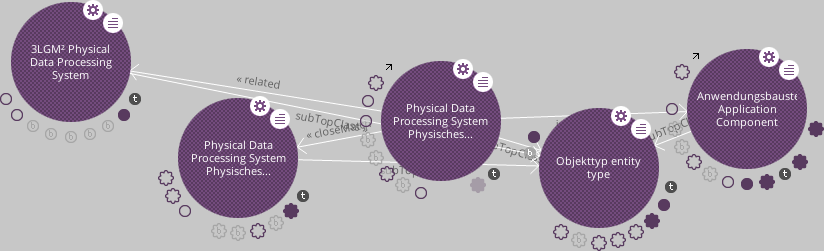
\includegraphics[width=0.95\textwidth]{img/lodlive.png}\\
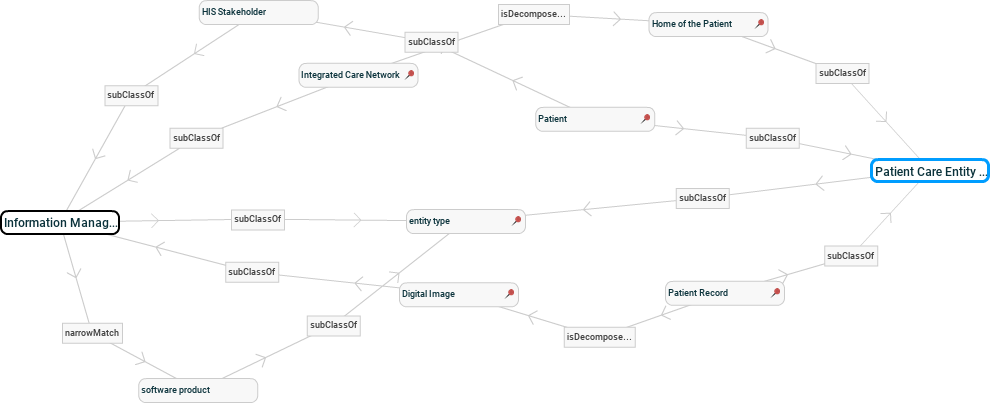
\includegraphics[width=0.95\textwidth]{img/relfinder.png}
\end{frame}
\fi
\iffalse
\section{Evaluieren}

\imageslide[https://imise.github.io/snik-ontology/2017/04/12/dashboard]{Statistiken}{img/dashboard-medley.png}{}{}
\imageslide[\url{https://github.com/IMISE/snik-ontology/issues}]{Ticketsystem}{img/gitissue.png}{}{}
\imageslide[\url{http://www.snik.eu/evaluation}]{TripleCheckMate}{img/triplecheckmate.png}{}{}

\section{Integrieren}

\imageslide[\url{http://www.snik.eu/sparql}]{SPARQL Endpoint}{img/sparqlresult.png}{}{}

\imageslide[http://aksw.org/Projects/LIMES]{LIMES}{img/limes.png}{}{}
\fi
\iffalse
\begin{frame}{Interlinking}
\begin{itemize}
\item Verknüpfungen zwischen Klassen verschiedener Ontologien
\item LIMES Tool von AKSW um Axel Ngonga
\item Finden von Kandidaten durch Stringähnlichkeit, manuelle Verifizierung und Kategorisierung
\end{itemize}
\end{frame}
\fi

\imageslide[https://github.com/IMISE]{Öffentliche Softwarerepositories}{img/github.png}{}{}

\section{Überblick}

\begin{frame}
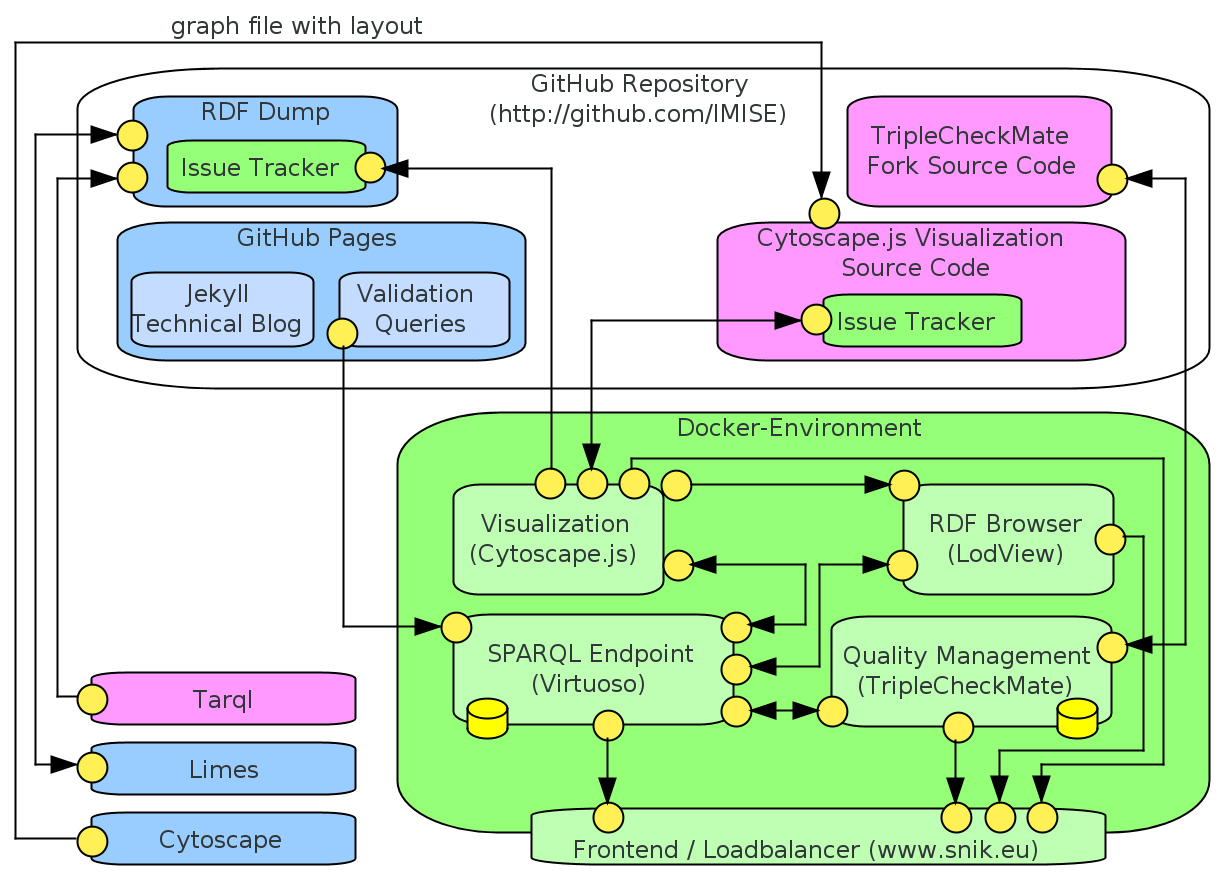
\includegraphics[width=\textwidth]{img/architecture.png}
\end{frame}

\begin{frame}[fragile]{Fragen?}
\begin{itemize}
%\item Diese Präsentation \url{https://github.com/KonradHoeffner/latex/releases/download/colloquium/colloquium.pdf}
\vspace{0.5em}%here it works as intended
\item Überblick \url{http://www.snik.eu}
\item Visualisierung \url{http://www.snik.eu/graph}
\item SPARQL Endpunkt \url{http://www.snik.eu/sparql}
\item RDF Browser \url{http://www.snik.eu/ontology}
\item Evaluation \url{http://www.snik.eu/evaluation}
\item Twitter \url{https://twitter.com/snik\_proj}
\item Technisches Blog \url{https://imise.github.io/snik-ontology}
\item GitHub Organisation mit Ticketsystem \url{https://github.com/imise}
\end{itemize}
\end{frame}

\end{document}
